\documentclass{article}
\usepackage[utf8]{inputenc}
\usepackage[margin=1in,includefoot]{geometry}

% Header and Footer Setup
\usepackage{fancyhdr}
\pagestyle{fancy}
\fancyhead{}
\fancyfoot{}
\fancyfoot[R]{\thepage}
\renewcommand{\headrulewidth}{0pt}
\renewcommand{\footrulewidth}{0pt}
%
%Graphics Setup
\usepackage{graphicx}
\usepackage{float}
\usepackage{subfig}

%list setup
\usepackage{amssymb}
\renewcommand{\labelitemi}{$\blacktriangleright$}
\renewcommand{\labelitemii}{$\bullet$}
\renewcommand{\labelitemiii}{$\circ$}

%Source Code setup
\usepackage{xcolor}
\usepackage{listings}

\definecolor{mGreen}{rgb}{0,0.6,0}
\definecolor{mGray}{rgb}{0.5,0.5,0.5}
\definecolor{mPurple}{rgb}{0.58,0,0.82}
\definecolor{backgroundColour}{rgb}{0.95,0.95,0.92}

\lstdefinestyle{CStyle}{
    backgroundcolor=\color{backgroundColour},   
    commentstyle=\color{mGreen},
    keywordstyle=\color{magenta},
    numberstyle=\tiny\color{mGray},
    stringstyle=\color{mPurple},
    basicstyle=\footnotesize,
    breakatwhitespace=false,         
    breaklines=true,                 
    captionpos=b,                    
    keepspaces=true,                 
    numbers=left,                    
    numbersep=5pt,                  
    showspaces=false,                
    showstringspaces=false,
    showtabs=false,                  
    tabsize=2,
    language=C
}
%


\begin{document}

\begin{titlepage}

	\begin{flushright}
	\textsc{\large March 24, 2021} \\
	\end{flushright}
	\begin{center}
	\Large{\bfseries GTU Department of Computer Engineering \\ CSE344 - Spring 2021 \\ Homework 1 Report  } \\
	\end{center}
	\topskip0pt
	\vspace*{\fill}
	\begin{center}
	\Large{\bfseries Akif Kartal \\ 171044098 }
	\end{center}
	\vspace*{\fill}

\end{titlepage}

\cleardoublepage
\section{Problem Definition}
The problem is to write an "advanced" file search program for POSIX compatible operating systems. 

\section{Solution}
In order to write this program we need to \textbf{divide problem into modules}. These modules are following;

\subsection{Argument Handling}
In order to manage arguments in a proper way I used \textbf{argument struct} to keep given argument data as one block data. My argument struct is following.
\begin{lstlisting}[style=CStyle]
typedef struct st
{
    int wFlag;
    int fFlag;
    int bFlag;
    int tFlag;
    int pFlag;
    int lFlag;
    char *wArg;
    char *fArg;
    char *bArg;
    char *tArg;
    char *pArg;
    char *lArg;
    int isFound;
    int count;

} args;
\end{lstlisting}
In this struct \textbf{count} represent number of optional arguments and \textbf{isFound} represent file is found or not.
Also, in order to get argument's value \textbf{getopt()} library method was used.
\subsection{Error Handling(Bonus)}
In order to handle any error \textbf{stderr} used with \textbf{write system call} and \textbf{exit} system call was used.
\begin{itemize}
	\item \textbf{Note:} In this part \textbf{fprintf library function was not used}. Instead write system call was used.
\end{itemize}
Following code shows an example of this;
\begin{lstlisting}[style=CStyle]
void my_fprintf_with_stderr(const char *str){
    ssize_t size = strlen(str);
    if (size != write(STDERR_FILENO, str, size)) {
        perror("write system call error!");
        exit(EXIT_FAILURE);
    }

}
\end{lstlisting}
\textbf{Usage:}
\begin{lstlisting}[style=CStyle]
if (closedir(dir))
{
    char *str = "Directory close error!!\n";
    my_fprintf_with_stderr(str);
    exit(EXIT_FAILURE);
} 
\end{lstlisting}
\subsection{Advanced Search Algorithm}
\subsubsection{Regex Handling}
The filename argument can contain more than one \textbf{"+"} character. To handle this situation in an easy way somehow we need to keep position data of these regexs. In order to do this I created my own \textbf{LinkedList} data structure to keep both position and previous letter information. \textbf{My LinkedList} node is following;
\begin{lstlisting}[style=CStyle]
//regex information node
typedef struct node_s
{
    int position;
    char preChr;
    struct node_s *next;

} node_t;
\end{lstlisting}
\subsubsection{Checking Given Parameters}
\begin{itemize}
	\item File name check was made by using regex linkedlist.
	\item File size, file type, file permissions and file links was checked by using \textbf{stat calls}. 
\end{itemize}
\subsubsection{Recursive Search Algorithm}
In this part we need to examine the files in the given target directory. In order to do this operation, we need to use \textbf{opendir} function.
Calling the opendir returns a \textbf{DIR*} type, which we will use to access the directory contents. After that we need to use \textbf{readdir} function with DIR* varible. Each time we call readdir, it returns a pointer to a \textbf{struct dirent} instance corresponding to the next directory entry.
The struct dirent that we get back from readdir has a field \textbf{d\textunderscore name}, which contains the name of the directory entry. So, in order to continue recursively traverse all directories, we need to use this d\textunderscore name file. After readdir call if directory is different than current and parent we will \textbf{concatenate "/" and d\textunderscore name end of the current directory name} after that when we call traversal function with this new path, we are able to examine and traverse inner directories. While making this also we need to check current file it is searched file or not. In order to do that we need to use  both d\textunderscore name and current path to use in stat function. Filename will be used checking filename flag. Lastly, we need close directory by calling \textbf{closedir} function, passing the DIR* type, to end the directory listing operation. Following \textbf{small code pieces} show this process.
\begin{lstlisting}[style=CStyle]
while ((entry = readdir(dir)) != NULL)
{
    //check directory is different than current and parent
    if (strcmp(entry->d_name, ".") != 0 && strcmp(entry->d_name, "..") != 0)
    {
        if (entry->d_type == DT_DIR)
        {
            checkGivenArguments(targetPath, givenArgs, entry->d_name);
            char currentPath[PATH_MAX];
            size_t size = strlen(targetPath);
            if (targetPath[size - 1] == '/')
                sprintf(currentPath, "%s%s", targetPath, entry->d_name);
            else
                sprintf(currentPath, "%s/%s", targetPath, entry->d_name);
            size_t pathLength = strlen(currentPath);
            traversePathRecursively(currentPath, givenArgs); //call function with child
        }
    }
}
//close directory
\end{lstlisting}

\subsubsection{Drawing nicely formatted tree}
If the searching file is found then directory tree will be drawn by using same recursive search algorithm with just a \textbf{minor} difference. 
\subsection{CTRL-C Handling}
In order to give a message on CTRL-C interrupt, I used \textbf{sigaction} function from \textbf{signal.h} library.
Also, I used a \textbf{global variable} to set if an interrupt has occur.
\begin{lstlisting}[style=CStyle]
volatile __sig_atomic_t exitSignal = 0;
void exitHandler(int signal)
{
    if (signal == SIGINT)
    {
        exitSignal = 1;
    }
}
\end{lstlisting}
In each loop in code, signal flag was checked, on interrupt signal, resources was given back and exited elegantly.
\section{Test Result}
A simple test result is following;
\begin{figure}[H]
    \centering
	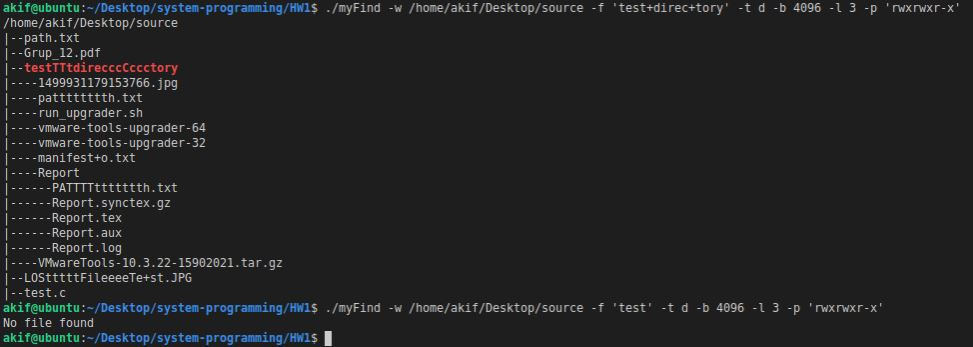
\includegraphics[width=7in, height=3in]{result.JPG}
	\caption[Optional caption]{}
	\label{}
\end{figure}                              

\end{document}